\documentclass[10pt,twocolumn,letterpaper]{article}

\usepackage{iccv}
\usepackage{times}
\usepackage{epsfig}
\usepackage{graphicx}
\usepackage{amsmath}
\usepackage{amssymb}

% Include other packages here, before hyperref.

% If you comment hyperref and then uncomment it, you should delete
% egpaper.aux before re-running latex.  (Or just hit 'q' on the first latex
% run, let it finish, and you should be clear).
\usepackage[pagebackref=true,breaklinks=true,letterpaper=true,colorlinks,bookmarks=false]{hyperref}

% \iccvfinalcopy % *** Uncomment this line for the final submission

\def\iccvPaperID{****} % *** Enter the ICCV Paper ID here
\def\httilde{\mbox{\tt\raisebox{-.5ex}{\symbol{126}}}}

% Pages are numbered in submission mode, and unnumbered in camera-ready
\ificcvfinal\pagestyle{empty}\fi

\begin{document}

%%%%%%%%% TITLE
\title{Representation Learning to Integrate Dynamic and Static Data for Improved Prediction on COVID-19 Patients Mortality}

\author{}

\maketitle
% Remove page # from the first page of camera-ready.
\ificcvfinal\thispagestyle{empty}\fi

%%%%%%%%% ABSTRACT
\begin{abstract}
   Seasonal influxes of COVID-19 infections put pressure on healthcare systems and make the allocation of limited resources and treatments extremely difficult. Because clinical measurements of COVID-19 patients can be collected over time, several longitudinal deep learning models have been proposed to predict clinical outcomes and aid in logistical decision making. These models often fail, however, to effectively handle missing data or integrate static data with the multivariate time series (MTS).We propose a novel semi-supervised learning framework that leverages Long Short-Term Memory (LSTM) to learn the vectorial representation of MTS which can be easily integrated with the static data. Using this representation, learned from both labeled and unlabeled samples, one can fully utilize the information in the MTS dataset. Experimental results utilizing chest X-ray images show that the proposed model significantly improves mortality classification compared to supervised models.
\end{abstract}

\iffalse
Mild cognitive impairment (MCI) is a transitional stage between age-related cognitive decline and Alzheimer’s disease (AD). For the effective treatment of AD, it would be important to identify MCI patients at high risk for conversion to AD. 
The novel characteristics of the methods for learning the biomarkers are as follows: 1) We used a semi-supervised learning method (low density separation) for the construction of MRI biomarker as opposed to more typical supervised methods; 2)
4) We constructed the aggregate biomarker by first learning a separate MRI biomarker and then combining it with age and cognitive measures about the MCI subjects at the baseline by applying a random forest classifier.
Alzheimer’s disease (AD), a common form of dementia, occurs most frequently in aged population. More than 30 million people worldwide suffer from AD and, due to the increasing life expectancy, this number is expected to triple by 2050 (The projected effect of risk factor reduction on Alzheimer's disease prevalence, Barnes DE).
Because of the dramatic increase in the prevalence of AD, the identification of effective biomarkers for the early diagnosis and treatment of AD in individuals at high risk to develop the disease is crucial.
Mild cognitive impairment (MCI) is a transitional stage between age-related cognitive decline and AD, and the earliest clinically detectable stage of progression towards dementia or AD (Neuropathologic alterations in mild cognitive impairment: a review, Markesbery WR). 
AD pathology has been therefore hypothesized to be detectable using neuroimaging techniques.(Neuropathologic alterations in mild cognitive impairment: a review, Markesbery WR)
Among different neuroimaging modalities, MRI has attracted a significant interest in AD related studies because of its completely non-invasive nature, high availability, high spatial resolution and good contrast between different soft tissues.
Clearly, predicting this disease in the early stages and preventing it from progressing is of great importance.
The diagnosis of Alzheimer’s disease (AD) requires a variety of medical tests, which leads to huge amounts of multivariate heterogeneous data. It can be difficult and exhausting to manually compare, visualize, and analyze this data due to the heterogeneous nature of medical tests; therefore, an efficient approach for accurate prediction of the condition of the brain through the classification of magnetic resonance imaging (MRI) images is greatly beneficial and yet very challenging. In this paper, a novel approach is proposed for the diagnosis of very early stages of AD through an efficient classification of brain MRI images
Next, using a small set of labeled training data,
The reason that early diagnosis of AD is of great importance is that the clinical therapies given to patients are much more effective in slowing down disease progression and helping preserve some cognitive functions of the brain if the patients are in the early stages of their disease.
In this paper, we propose a novel method for a high-level latent and shared feature representation from neuroimaging modalities via deep learning. 
Furthermore, fusing the complementary information from multiple modalities helps enhance the diagnostic accuracy[Identification of conversion from mild cognitive impairment to Alzheimer's disease using multivariate predictors.; Multivariate examination of brain abnormality using both structural and functional MRI.]
To this end, many researchers have devoted their efforts to find biomarkers and develop a computer-aided system, with which we can effectively predict or diagnose the diseases.
In a semi-supervised method, feature vectors from unlabeled data are also used in the learning process in addition to the labels and feature vectors from the labeled ones.
\fi

\section{Introduction}
% Why our model is good? : (1) Semi-supervised learning -> Our model can learn from labeled/unlabeled samples BOTH. (2) Learn temporal trends from the time series with missing records (MRI imagings are captured inconsistently (the number of records/the time points of records are different) from the participants). (3) Combine the multi-modal (genotypic modality (SNPs, static) + phenotypic (neuroimagings, dynamic) modality) data with two Autoencoders: one for static, another for time series.
% Find the related works with the lack of above advantages of our model.
\section{Methods}
\iffalse
% retaining as much useful information as possible to allow an accurate reconstruction [hinton2006reducing].
Why should this learn good features? In order to predict the next few frames correctly, the model needs information about which objects and background are present and how they are moving so that the motion can be extrapolated. The hidden state coming out from the encoder will try to capture this information. Therefore, this state can be seen as a representation of the input sequence.
The two tasks – reconstructing the input and predicting the future can be combined to create a composite model as shown in Fig. 4.

Broadly speaking, an autoencoder system is a generative model comprised of an encoder and a decoder module that are sequentially connected together. Consequently, the input to such a system is a set of signals following a certain distribution, i.e. x ∼ P(x), and the output is the recovered signal xˆ from the decoder module using the latent representations. In short, the goal is to jointly learn an abstract representation of the underlying distribution of the signals through the encoder module, and simultaneously, learning a decoder module allowing for reconstruction of the input signals from the obtained abstract representations
\fi
%%%%%%%%%%%%%%%%%%%%%%%%%%%%%%%%%%%%%%%%%%%%%%%%%%%%%%%%%%%%%%%%%%%%%%%%%%%%%%%%%%%
In this section, we describe the structure of proposed autoencoder (AE) which is a composite model of three components. The LSTM encoder $\phi_E$ encodes the longitudinal record of each patient into the enriched representation. The multilayer perceptron (MLP) decoder $\phi_D$ decodes the enriched representation into the original record. The MLP predictor $\phi_P$ predicts the target labels from the enriched representation. The input and output of the proposed model is described in Fig.~\ref{fig: LSTM and MLP}.
\begin{figure*}
    \centering
    \includegraphics[width=1.0\textwidth]{figures/network-structure.png}
    \caption{The workflows of the enrichment learning task. The enriched representation at the bottleneck of the LSTM autoencoder is used to reconstruct the longitudinal records and predict the mortality.} \label{fig: LSTM and MLP}
\end{figure*}

\subsection{Dataset}
% Normalized, Min-max scaling. Time point to floating numbers, seconds after admission.
We obtain the blood sample records, demographic information, and associated mortality outcomes of 375 patients collected throughout their stay in Tongji hospital between 10th January and 24th February 2020 following the previous research~\cite{yan2020interpretable}. We discard 17 samples whose no time stamp is recorded. Among the remaining 358 samples, 192 patients survived (labeled as 1) and 166 patients died (labeled as 0). The order of samples is randomly shuffled to prevent the bias from the order. Each feature of dataset is normalized by min-max scaling to the range [0, 1]. 

\subsection{Notations}
In this paper, we denote a vector as a bold lower case letter, and matrix as a bold upper case letter. 
% For the arbitrary matrix $\mathbf{X}$, $\mathbf{x}^r$, $\mathbf{x}_c$, $x^r_c$ denotes the $r$-th row, $c$-th column, an element of $r$-th row and $c$-th column respectively. 
We use $i$ and $j$ to index $i$-th participant and $j$-th record respectively. We describe the records of $i$-th participant as $\mathcal{X}_i = \{\mathbf{x}_i^b, \mathbf{X}_i, \mathbf{M}_i, \mathbf{t}_i\}$ as follows:
\begin{itemize}
    \item $\mathbf{x}_i^b \in \Re^{D_b}$ is a vector of basic demographic information, such as age and gender.
    \item $\mathbf{X}_i = [\mathbf{x}_i^1; \mathbf{x}_i^2; \cdots; \mathbf{x}_i^{n_i}] \in \Re^{n_i \times D_l}$ are the longitudinal records collected from the blood tests across the $n_i$ time points.
    \item $\mathbf{M}_i = [\mathbf{m}_i^1; \mathbf{m}_i^2; \cdots; \mathbf{m}_i^{n_i}] \in \{1, 0\}^{n_i \times D_l}$ are the binary masks of observabilities of longitudinal records $\mathbf{X}_i$, where 1 and 0 indicates the observed and unobserved entry respectively.
    \item $\mathbf{t}_i = [t_i^1; t_i^2; \cdots; t_i^{n_i}] \in \Re^{n_i}$ are the time stamps of $n_i$ records.
\end{itemize}
The missing entries in $\mathbf{X}_i$ are initialized with the constant $-1$, and this value does not affect the result. The target label $\mathbf{y}_i \in \{0, 1\}$ is the mortality of $i$-th participant, which is provided in the training process if that participant is in training set, such that $i \in \Omega$.

\subsection{Encoder}
We leverage LSTM encoder $\phi_{E}: \Re^{n_i \times (2 D_l + 1)} \mapsto \Re^{d_z}$ to summarize the longitudinal records and learn the temporal relation between records. The time stamp of each record is crucial in learning the temporal relation between records (e.g. temporal locality), while the the missingness pattern of the entries may represent the participants' status. Thus we provide the concatenation of longitudinal records, masks, and time stamps, $[\mathbf{X}_i, \mathbf{M}_i, \mathbf{t}_i] = [\hat{\mathbf{x}}_i^1; \hat{\mathbf{x}}_i^2; \cdots; \hat{\mathbf{x}}_i^{n_i}] = \hat{\mathbf{X}}_i \in \Re^{n_i \times (2 D_l + 1)}$, as an input of LSTM encoder such that $\phi_{E}(\mathbf{X}_i, \mathbf{M}_i, \mathbf{t}_i;\ \theta_E) = \mathbf{z}_i$. Here, $\theta_E$ denotes the set of trainable parameters of LSTM.

For each time step ($1 \leq j \leq n_i$), the input record $\hat{\mathbf{x}}_i^j$ of $i$-th patient is processed by following the LSTM architecture~\cite{yu2019review}:
\begin{equation}
    \mathbf{k}^j_i = \sigma(\hat{\mathbf{x}}^j_i \mathbf{W}_{xk} + \mathbf{h}_i^{j-1} \mathbf{W}_{hk} + \mathbf{c}_i^{j-1} \mathbf{W}_{ck} + \mathbf{b}_k),
\end{equation}
\begin{equation}
    \mathbf{f}^j_i = \sigma(\hat{\mathbf{x}}^j_i \mathbf{W}_{xf} + \mathbf{h}^{j-1}_i \mathbf{W}_{hf} + \mathbf{c}^{j-1}_i \mathbf{W}_{cf} + \mathbf{b}_f),
\end{equation}
\begin{equation}
    \mathbf{c}^j_i = \mathbf{f}^j_i \odot \mathbf{c}^{j-1}_i + \mathbf{k}^j_i \odot \operatorname{tanh}(\hat{\mathbf{x}}_i^j \mathbf{W}_{xc} + \mathbf{h}^{j - 1}_i \mathbf{W}_{hc} + \mathbf{b}_c),
\end{equation}
\begin{equation}
    \mathbf{o}^j_i = \sigma(\hat{\mathbf{x}}_i^j \mathbf{W}_{xo} + \mathbf{h}^{j-1}_i \mathbf{W}_{ho} + \mathbf{c}^j_i \mathbf{W}_{co} + \mathbf{b}_o),
\end{equation}
\begin{equation}
    \mathbf{h}^j_i = \mathbf{o}^j_i \odot \operatorname{tanh}(\mathbf{c}^j_i),
\end{equation}
where $\sigma$ and tanh is the logistic sigmoid and hyperbolic tangent activation function respectively, and $\mathbf{k}^j_i$, $\mathbf{o}^j_i$, $\mathbf{f}^j_i$ are input, output, forget gate of $j$-th time step respectively. \{$\mathbf{W}_{xk}$, $\mathbf{W}_{hk}$, $\mathbf{W}_{ck}$, $\mathbf{W}_{xf}$, $\mathbf{W}_{hf}$, $\mathbf{W}_{cf}$, $\mathbf{W}_{xc}$, $\mathbf{W}_{hc}$, $\mathbf{W}_{xo}$, $\mathbf{W}_{ho}$, $\mathbf{W}_{co}$\} $\subset \mathbf{\theta}_E$ are trainable weight matrices and $\{\mathbf{b}_k, \mathbf{b}_f, \mathbf{b}_c, \mathbf{b}_o\} \subset \mathbf{\theta}_E$ are trainable bias vectors. $\mathbf{c}_i^j$ and $\mathbf{h}_i^j$ denote the cell state and hidden representation at $j$-th time step. The hidden representation $\mathbf{h}_i^{n_i}$ at the last time step $n_i$ is our enriched representation of the longitudinal records $\hat{\mathbf{X}}_i$, such that $\mathbf{h}_i^{n_i} = \mathbf{z}_i \in \Re^{d_z}$.
\begin{equation}
    \mathbf{h}_i^{n_i} = \mathbf{z}_i = \phi_E(\mathbf{X}_i, \mathbf{M}_i, \mathbf{t}_i; \mathbf{\theta}_E).
\end{equation}
Since the hidden representation at $j$-th time point aims to summarize the records from first time step to $j$-th time step, the LSTM cell needs to refer to the cell state $\mathbf{c}_i^j$ and reflect past records to $\mathbf{h}_i^j$. Since the cell state $\mathbf{c}_i^j$ is guided by the input gate $\mathbf{k}_i^j$ and forget gate $\mathbf{f}_i^j$, which control how much information came from previous step should be preserved, the cell state $\mathbf{c}_i^j$ enables the hidden representation $\mathbf{h}_i^j$ to learn long term dependencies. For example, LSTM encoder can capture the temporal trends of patient's status from the consecutive records.

% \subsubsection{Autoencoder}
% The encoder $\phi: \Re^{n_i \times (2 D_l + 1)} \mapsto \Re^{D_z}$ maps the input MTS in the high dimensional space into the latent representation in the lower dimensional space, such that $\phi_E(\mathbf{X}_i, \mathbf{M}_i, \mathbf{t}_i; \mathbf{\theta}_E) = \mathbf{z}_i \in \Re^{D_z}$. From the enriched representation $\mathbf{z}_i$, decoder $\phi_D: \Re^{D_z + 1} \mapsto \Re^{D_l}$ reconstructs the original record $\phi_D(\mathbf{z}_i ,t_i^j; \mathbf{\theta}_D) = \tilde{\mathbf{x}}_i^j \in \Re^{D_l}$, for each time point $t_i^j$ ($1 \leq j \leq n_i$). The predictor $\phi_P: \Re^{D_z + D_b} \mapsto [0, 1]$ generates the prediction $\phi_P(\mathbf{z}_i, \mathbf{x}_i^b; \mathbf{\theta}_P) = \tilde{y}_i$. $D_b, D_l, D_z$ denote the dimensionality of static, longitudinal, enriched biomarkers, and $\mathbf{\theta}_E, \mathbf{\theta}_D, \mathbf{\theta}_P$ denote the trainable parameters of encoder, decoder, predictor, respectively. 
% % Then we combine encoder, decoder, and predictor as a composite model, illustrated in Fig.~\ref{fig: autoencoder}.

% \subsection{Encoder}
% We leverage an LSTM encoder to compress MTS and extract long term dependencies in the temporal trend. 
% \subsubsection{Input}
% Because the time stamp of each record is crucial to learn the temporal trend and missingness pattern of the entries may represent the state of patient, we provide the concatenation of longitudinal records, masks, and time stamps $[\mathbf{X}_i, \mathbf{M}_i, \mathbf{t}_i] = \hat{\mathbf{X}}_i = [\hat{\mathbf{x}}_i^1; \hat{\mathbf{x}}_i^2; \cdots; \hat{\mathbf{x}}_i^{n_i}] \in \Re^{n_i \times (2 D_l + 1)}$ to the input layer of LSTM encoder. 
% The inputs of LSTM are $\hat{\mathbf{x}}_i^j$, $\mathbf{h}_{j - 1}$, $\mathbf{c}_{j - 1}$ and outputs are $\mathbf{h}_{j}$ and $\mathbf{c}_{j}$, where $\mathbf{h}_{j}$ is the hidden representation of records and $\mathbf{c}_{j}$ is the cell state of LSTM cell at $j$-th time step. 

% \subsubsection{Output}
% For each time step ($1 \leq j \leq n_i$), the input record $\hat{\mathbf{x}}_i^j$ of $i$-th patient is processed by following the LSTM architecture~\cite{yu2019review}:
% % The hidden representation $\mathbf{h}_j$ should compress the longitudinal records from first time step to $j$-th time step to accurately reconstruct the records, and the final hidden representation $\mathbf{h}_{n_i} = \mathbf{z}_i$ is the encoded representation of longitudinal records.
% \begin{equation}
%     \mathbf{k}^j_i = \sigma(\hat{\mathbf{x}}^j_i \mathbf{W}_{xk} + \mathbf{h}_i^{j-1} \mathbf{W}_{hk} + \mathbf{c}_i^{j-1} \mathbf{W}_{ck} + \mathbf{b}_k),
% \end{equation}
% \begin{equation}
%     \mathbf{f}^j_i = \sigma(\hat{\mathbf{x}}^j_i \mathbf{W}_{xf} + \mathbf{h}^{j-1}_i \mathbf{W}_{hf} + \mathbf{c}^{j-1}_i \mathbf{W}_{cf} + \mathbf{b}_f),
% \end{equation}
% \begin{equation}
%     \mathbf{c}^j_i = \mathbf{f}^j_i \odot \mathbf{c}^{j-1}_i + \mathbf{k}^j_i \odot \operatorname{tanh}(\hat{\mathbf{x}}_i^j \mathbf{W}_{xc} + \mathbf{h}^{j - 1}_i \mathbf{W}_{hc} + \mathbf{b}_c),
% \end{equation}
% \begin{equation}
%     \mathbf{o}^j_i = \sigma(\hat{\mathbf{x}}_i^j \mathbf{W}_{xo} + \mathbf{h}^{j-1}_i \mathbf{W}_{ho} + \mathbf{c}^j_i \mathbf{W}_{co} + \mathbf{b}_o),
% \end{equation}
% \begin{equation}
%     \mathbf{h}^j_i = \mathbf{o}^j_i \odot \operatorname{tanh}(\mathbf{c}^j_i),
% \end{equation}
% where $\sigma$ is logistic sigmoid activation function and $\mathbf{k}^j_i$, $\mathbf{o}^j_i$, $\mathbf{f}^j_i$ are input, output, forget gate of $j$-th time step respectively. \{$\mathbf{W}_{xk}$, $\mathbf{W}_{hk}$, $\mathbf{W}_{ck}$, $\mathbf{W}_{xf}$, $\mathbf{W}_{hf}$, $\mathbf{W}_{cf}$, $\mathbf{W}_{xc}$, $\mathbf{W}_{hc}$, $\mathbf{W}_{xo}$, $\mathbf{W}_{ho}$, $\mathbf{W}_{co}$\} $\subset \mathbf{\theta}_{E}$ are trainable weights matrix and $\{\mathbf{b}_k, \mathbf{b}_f, \mathbf{b}_c, \mathbf{b}_o\} \subset \mathbf{\theta}_{E}$ are trainable bias vectors. $\mathbf{c}_i^j$ and $\mathbf{h}_i^j$ denote the cell state and hidden representation. 

% In order decoder and predictor to reconstruct the original record and predict the target label accurately, the enriched representation should contain enough information for reconstruction and prediction, such as temporal trend of input sequence. The goal of encoder at $j$-th time pont is to generate the hidden representation $\mathbf{h}_i^j$ summarizing the records from first time step to $j$-th time step, therefore the LSTM cell refers to the cell state $\mathbf{c}_i^j$ and reflect the past records to $\mathbf{h}_i^j$. Since the cell state $\mathbf{c}_i^j$ is guided by the input gate $\mathbf{k}_i^j$ and forget gate $\mathbf{f}_i^j$ which control how much information came from previous step should be preserved, the cell state $\mathbf{c}_i^j$ enables the hidden representation $\mathbf{h}_i^j$ to learn the long term dependencies. For example, if the differences in the records and time intervals between the time points of recent 10 consecutive records are small, the hidden representation of 10 time steps before can be preserved.
% % and  and  Because input gate $\mathbf{k}_i^j$ and forget gate $\mathbf{f}_i^j$ control how much we keep the information came from previous step, therefore LSTM is able to convey the most useful inf
% The hidden representation $\mathbf{h}_i^{n_i}$ at the most recent time point is the enriched representation $\mathbf{z}_i$ of whole longitudinal records of $i$-th patent:
% % Then the enriched representation $\mathbf{z}_i$ is given to the decoder and predictor.
% \begin{equation}
%     \mathbf{h}_i^{n_i} = \mathbf{z}_i = \phi_E(\mathbf{X}_i, \mathbf{M}_i, \mathbf{t}_i; \mathbf{\theta}_E).
% \end{equation}

\subsection{Decoder and Predictor}
From the enriched representation $\mathbf{z}_i$ of longitudinal records, the decoder reconstruct the original record, and predictor predicts the target label.
The decoder and predictor both are the multilayer perceptron (MLP), instead of LSTM. A previous study~\cite{srivastava2015unsupervised} that attempted to enrich longitudinal records with a recurrent neural network (RNN)~\cite{medsker2001recurrent}, did so by using RNNs for both the encoder and decoder, where the output (reconstructed record) of the decoder at each time step depends on the output at the previous time step. However, since no additional information is provided to the decoder other than a learned representation that is no longer longitudinal, there should not be dependency between the outputs of the decoder. Because the enriched representation $\mathbf{z}_i$ summarizes \emph{whole} longitudinal records, the decoder $\phi_D:\Re^{d_z + 1} \mapsto \Re^{D_l}$ should be able to reconstruct the $j$-th record $\mathbf{x}_i^j$ given time stamp $t_i^j$ without any additional information, such that $\phi_D(\mathbf{z}_i, t^j_i;\ \theta_D) = \tilde{\mathbf{x}}_i^j \approx \mathbf{x}_i^j$, where $\theta_D$ is a set of weight matrices and bias vectors of the decoder. This autoencoder architecture, to the best of our knowledge, has not yet been proposed. 

MLP consists of the consecutive hidden layers as follows:
\begin{equation}
    \mathbf{h}_k = \sigma(\mathbf{W}_k\mathbf{h}_{k-1} + \mathbf{b}_k),
\end{equation}
where $\mathbf{h}_k$ is the output of $k$-th hidden layer, and $\sigma$ is the activation function, and $\mathbf{W}_k$, $\mathbf{b}_k$ are the trainable weights matrix and bias vector of $k$-th hidden layer. The output is earned by forwarding the input vector $\mathbf{h}_0$ to the last hidden layer. To recover the original record at the specific time point, the decoder needs to know that time point. Thus the input vector of decoder is the concatenation of enriched representation $\mathbf{z}_i$ and time stamp $t^j_i$, which is $[\mathbf{z}_i, t_i^j] \in \Re^{d_z + 1}$. For predictor, the demographic information such as age may be crucial to predict target label. Therefore we provide the demographic information to the predictor with the enriched representation, which is $[\mathbf{z}_i, \mathbf{x}_i^b] \in \Re^{d_z + D_b}$. By forwarding each input of decoder and predictor to their own MLP, we earn the reconstructed record $\tilde{\mathbf{x}}_i^j$ and prediction $\tilde{y}_i$ on target label:
\begin{equation}
    \phi_D(\mathbf{z}_i, t_i^j; \mathbf{\theta}_D) = \tilde{\mathbf{x}}_i^j,
\end{equation}
\begin{equation}
    \phi_P(\mathbf{z}_i, \mathbf{x}_i^b; \mathbf{\theta}_P) = \tilde{\mathbf{y}}_i,
\end{equation}
and we have the stack of reconstructed records of $i$-th patient:
\begin{equation}
    \tilde{\mathbf{X}}_i = [\tilde{\mathbf{x}}_i^1; \tilde{\mathbf{x}}_i^2; \cdots; \tilde{\mathbf{x}}_i^{n_i}].
\end{equation}
\begin{figure*}[t]
    \centering
    \includegraphics[width=0.9\textwidth]{figures/autoencoder.pdf}
    \caption{An illustration for the loss functions. The encoder consists of LSTM cell, which processes input record $\mathbf{x}_i^j$, and then generates the hidden representation $\mathbf{h}_i^j$ while conveying the cell state $\mathbf{c}_i^j$ to the next step. The enriched representation of the whole time series is defined as the hidden representation $\mathbf{h}_i^{n_i}$ at the last step.} \label{fig: autoencoder}
\end{figure*}
% \begin{equation}
%     \mathbf{\tilde{x}}_i^j = \sigma(\mathbf{W}_3 \sigma(\mathbf{W}_2 \sigma(\mathbf{W}_1 [\mathbf{z}_i, t_i^j] + \mathbf{b}_1) + \mathbf{b}_2) + \mathbf{b}_3) \sigma(\mathbf{W}_k\mathbf{h}_{k-1} + \mathbf{b}_k)
% \end{equation}
% In other words, the decoder should be able to reconstruct the original record with enriched vectorial representation $\mathbf{z}_i$ and time stamp $t_i^j$ if $\mathbf{z}_i$ successfully summarizes the records of all time steps. 

\subsection{Loss Functions}
AE is asked to accomplish the two tasks - reconstructing original records and predicting target label by minimizing:
\begin{equation}\label{eq: objective}
    \min_{\theta_E, \theta_D, \theta_P} \mathcal{L}_{total} = \min_{\theta_E, \theta_D, \theta_P}(\gamma_1\mathcal{L}_{reconstruct} + \gamma_2\mathcal{L}_{predict}),
\end{equation}
where $\gamma_1$ and $\gamma_2$ are the hyperparameters to adjust the impact of each loss.
The reconstruction loss is defined as the scaled Mean Squared Error (MSE):
\begin{equation}
    \mathcal{L}_{reconstruct} = \frac{\left\| (\tilde{\mathbf{X}}_i - \mathbf{X}_i) \odot \mathbf{M}_i \right\|_F^2}{|\mathbf{M}_i|},
\end{equation}
where squared Frobenious norm $\| \cdot \|_F^2$ is defined as the summation of all the entries squared.

The the prediction loss is defined respect to the labeled $i \in \Omega$ and unlabeled $i \not\in \Omega$ data separately:
\begin{equation}
    \mathcal{L}_{predict} = \left\{\begin{array}{lr}
        \| \tilde{y}_i - y_i \|_F^2, & \text{for } i \in \Omega\\
        0, & \text{for } i \not\in \Omega
    \end{array}\right\}.
\end{equation}
The high capacity unsupervised AE may suffer from the tendency to learn the trivial identity mapping and memorize the input~\cite{srivastava2015unsupervised}. The addition of prediction loss can prevent this memorization problem, because the memorization is not useful to predict the target label.

%Here the encoder LSTM is asked to come up with a state from which we can both predict the next few frames as well as reconstruct the input.
% This composite model tries to overcome the shortcomings that each model suffers on its own. A high-capacity autoencoder would suffer from the tendency to learn trivial representations that just memorize the inputs. However, this memorization is not useful at all for predicting the future. Therefore, the composite model cannot just memorize information.

% $L_{pred}$ is 0 when test set.
% Structure of LSTM, and if decoder is LSTM, then which state should be passed?
% Image for input (static + dynamic concatenation) and output (RE\_DATE is concatenated), and prediction target.
% LSTM unit explanation with maybe Figure. Concatenate static features because they are helpful to learn enrichment.
% Figure : Balance, reconstruction error vs prediction error.
% Why decoder is not RNN? Think of what is input for encoder and decoder. Because there is no information is additionally provided, current prediction depends on previous prediction does not make sense. The enriched representation is the fixed-length vector which is not longitudinal records anymore.
\iffalse
Data used in this work include all subjects for whom baseline MRI data (T1-weighted MP-RAGE sequence at 1.5 T, typically 256 × 256 × 170 voxels with the voxel size of approximately 1 mm × 1 mm × 1.2 mm), at least moderately confident diagnoses (i.e. confidence > 2), hippocampus volumes (i.e. volumes of left and right hippocampi, calculated by FreeSurfer Version 4.3), and test scores in certain cognitive scales (i.e. ADAS: Alzheimer’s Disease Assessment Scale, range 0–85; CDR-SB: Clinical Dementia Rating ‘sum of boxes’, range 0–18; MMSE: Mini-Mental State Examination, range 0–30) were available.
Because one of the primary goals of our regression analysis is to identify a subset of imaging markers which are highly correlated to the AD progression reflected by the cognitive changes over time.
In summary, the identified longitudinally stable imaging markers are highly suggestive and strongly agree with the existing research findings,

The time points examined in this study for both imaging biomarkers and cognitive assessments include the baseline (BL), the 6th month (M6), the 12th month (M12), the 18th month (M18), the 24th month (M24) and the 36th month (M36).

As a result, a total of 544 sample subjects are selected in our study, among which 92 samples are diagnosed with AD, 205 samples are diagnosed to be with Mild Cognitive Impairment (MCI), and 177 samples are HC.

From the top panel of Fig. 4 we can see that the VBM biomarkers with highest weights are perfectly in accordance with existing medical findings. Specifically, we observe that the bilateral hippocampus are among the top selected biomarkers. In addition, the bilateral amygdala is also among the top selected biomarkers. Finally, We notice that the bilateral putamen are also among the top selected biomarkers. , which is one more indication of the correctness our new method.
Specifically, if the number of labeled images is small, semi-supervised approach appears to yield higher classification accuracy.
\fi

\section{Experiments} % 3.5 pages length recommended.
% The distribution of a feature may be categorized -> swap is better than gradient.
Our experiments consist of two parts: (1) we compare the prediction performance of the proposed model to the widely used prediction models, and (2) we identify the biomarkers which are most predictive for AD progression.
% We use AD progression in AD, MCI and HC as predictive targets in our studies.
% Although their deep learning approaches have shown the promising prediction results in binary classifications, but multi-class models have not achieved enough accuracy for clinical applicability.
\subsection{Classification Performance}
\subsubsection{Competing models}
For an ablation study to observe the effectiveness of our semi-supervised autoencoder (SAE), we introduce a baseline LSTM (BLSTM) model by removing decoders $\psi_{SNP}$ and $\psi_{dynamic}$ from our model SAE. In addition to the longitudinal model, we use the random forest~\cite{ho1995random} (RF) with 34 max depth and deep neural network (DNN) with 5 fully connected layers. Since these competing models are not longitudinal, we provide the concatenation of the most recent record $[\mathbf{x}_i^b, \mathbf{x}_i^s, \mathbf{x}_i^{n_i}]$ to them. Both the training and test sets are provided to train SAE in a semi-supervised manner, while the other competing models are trained only with the training set. Although the order of participants is randomly shuffled to avoid the bias, we use the same training and test data across all the competing methods for a fair comparison. The hyperparameters of our model are provided in the supplementary.
\subsubsection{Result and Evaluation}
We conduct the multiclass AD progression prediction task for 1 year ahead.
% \begin{equation}\label{eq: metrics}
% \begin{aligned}
%     &\text{Accuracy} = \frac{\sum_{c \in C}(TP_c + TN_c)}{\sum_{c \in C}(TP_c + TN_c + FP_c + FN_c)},\\
%     &\text{Precision of class }c=\frac{TP_c}{TP_c + FP_c},\ \text{Recall of class }c=\frac{TP_c}{TP_c+FN_c},
% \end{aligned}
% \end{equation}
% where $C$ is a set of classes \{AD, MCI, HC\}.
In table~\ref{tab: experimetal results}, the average and standard deviation of performance results across $k$ groups are reported following a $k$-fold cross validation scheme. We split the dataset into $k=2,\ 3,\ 5$ subgroups, such that 50\%, 66\%, 80\% of participants belong to the training set respectively. In table~\ref{tab: experimetal results}, nan (not a number) in precision on specific class means the model never predicted that class in one of $k$ subgroups.
% Considering the prediction of random forest is biased towards AD (high AD Recall), our model SAE generally outperforms other competing models. Interestingly, the performance gap between SAE and BLSTM increases as the size of training set decreases. 
Our model SAE generally outperforms other competing models especially when the proportion of training set is small. We suppose that this is because our semi-supervised learning approach can learn from the unlabeled samples in test set, while the other models cannot. This finding shows our model's promise in the early diagnosis of AD.
% This finding shows our model's versatility in handling samples, as well as its promise in the early diagnosis of AD.
% [Emphasize AD precision, recall as it is good, and important to detect than MCI and HC, can detect characteristics of the samples of AD participant.]

\begin{table*}[ht]
    \centering
    \caption{The prediction performance from k-fold cross validation. Receiver operating characteristic curves of this result is provided in supplementary.}\label{tab: experimetal results}
    \begin{tabular}{c c cccc}
        \toprule
    \multirow{1}{*}{\bfseries Training Set} & {\bfseries Metric} & \multicolumn{1}{c}{{\bfseries SAE} (Ours)} & \multicolumn{1}{c}{{\bfseries BLSTM}} & \multicolumn{1}{c}{{\bfseries RF}} & {\bfseries DNN}         \\
    \midrule
    \multirow{7}{*}{80\%} %% 7 rows group.
    & Accuracy & \multicolumn{1}{c}{{\bfseries 74.95$\pm$4.72}} & \multicolumn{1}{c}{71.57$\pm$5.29} & \multicolumn{1}{c}{71.79$\pm$6.33} & 49.45$\pm$2.91\\
    & AD Precision & \multicolumn{1}{c}{{\bfseries 71.28$\pm$11.89}} & \multicolumn{1}{c}{71.19$\pm$16.79} & \multicolumn{1}{c}{70.55$\pm$9.22} & 55.13$\pm$6.30\\
    & MCI Precision & \multicolumn{1}{c}{59.84$\pm$10.11} & \multicolumn{1}{c}{{\bfseries 60.07$\pm$11.74}} & \multicolumn{1}{c}{59.64$\pm$8.15} & 33.84$\pm$4.97\\
    & HC Precision & \multicolumn{1}{c}{{\bfseries 89.69$\pm$7.33}} & \multicolumn{1}{c}{86.60$\pm$8.15} & \multicolumn{1}{c}{87.28$\pm$9.88} & 47.02$\pm$7.9\\
    & AD Recall & \multicolumn{1}{c}{69.30$\pm$7.30} & \multicolumn{1}{c}{65.92$\pm$21.31} & \multicolumn{1}{c}{{\bfseries 71.18$\pm$12.64}} & 74.49$\pm$7.45\\
    & MCI Recall & \multicolumn{1}{c}{{\bfseries 66.00$\pm$11.83}} & \multicolumn{1}{c}{60.00$\pm$8.57} & \multicolumn{1}{c}{61.47$\pm$11.93} & 22.89$\pm$2.93\\
    & HC Recall & \multicolumn{1}{c}{85.36$\pm$8.98} & \multicolumn{1}{c}{{\bfseries 89.37$\pm$6.53}} & \multicolumn{1}{c}{86.58$\pm$9.50} & 36.33$\pm$8.67\\
    \midrule
    \multirow{7}{*}{66\%} %% 7 rows group.
    & Accuracy & \multicolumn{1}{c}{{\bfseries 73.34$\pm$1.71}} & \multicolumn{1}{c}{69.92$\pm$1.94} & \multicolumn{1}{c}{61.83$\pm$4.02} & 47.81$\pm$1.65\\
    & AD Precision & \multicolumn{1}{c}{{\bfseries 63.47$\pm$7.84}} & \multicolumn{1}{c}{62.10$\pm$5.53} & \multicolumn{1}{c}{51.63$\pm$1.29} & 55.26$\pm$1.61\\
    & MCI Precision & \multicolumn{1}{c}{{\bfseries 63.97$\pm$8.74}} & \multicolumn{1}{c}{55.39$\pm$7.85} & \multicolumn{1}{c}{53.91$\pm$8.85} & 31.03$\pm$1.37\\
    & HC Precision & \multicolumn{1}{c}{{\bfseries 88.62$\pm$3.47}} & \multicolumn{1}{c}{85.94$\pm$3.09} & \multicolumn{1}{c}{71.74$\pm$3.14} & 46.64$\pm$6.77\\
    & AD Recall & \multicolumn{1}{c}{{\bfseries 69.14$\pm$6.16}} & \multicolumn{1}{c}{63.90$\pm$7.23} & \multicolumn{1}{c}{59.48$\pm$8.8} & 70.09$\pm$6.63\\
    & MCI Recall & \multicolumn{1}{c}{{\bfseries 56.97$\pm$8.32}} & \multicolumn{1}{c}{53.85$\pm$10.16} & \multicolumn{1}{c}{39.09$\pm$11.54} & 27.62$\pm$5.09\\
    & HC Recall & \multicolumn{1}{c}{{\bfseries 88.55$\pm$3.44}} & \multicolumn{1}{c}{85.48$\pm$3.04} & \multicolumn{1}{c}{36.56$\pm$2.84} & 32.44$\pm$6.52\\
    \midrule
    \multirow{7}{*}{50\%} %% 7 rows group.
    & Accuracy & \multicolumn{1}{c}{{\bfseries 72.29$\pm$2.44}} & \multicolumn{1}{c}{47.29$\pm$23.60} & \multicolumn{1}{c}{53.69$\pm$2.04} & 47.68$\pm$0.13\\
    & AD Precision & \multicolumn{1}{c}{{\bfseries 60.79$\pm$2.25}} & \multicolumn{1}{c}{50.38$\pm$26.69} & \multicolumn{1}{c}{51.56$\pm$2.68} & 52.87$\pm$2.26\\
    & MCI Precision & \multicolumn{1}{c}{{\bfseries 60.93$\pm$6.38}} & \multicolumn{1}{c}{nan$\pm$nan} & \multicolumn{1}{c}{nan$\pm$nan} & 33.12$\pm$6.56\\
    & HC Precision & \multicolumn{1}{c}{{\bfseries 86.99$\pm$2.20}} & \multicolumn{1}{c}{nan$\pm$nan} & \multicolumn{1}{c}{64.99$\pm$2.28} & 44.38$\pm$0.06\\
    & AD Recall & \multicolumn{1}{c}{72.90$\pm$8.45} & \multicolumn{1}{c}{81.36$\pm$18.64} & \multicolumn{1}{c}{{\bfseries 98.14$\pm$0.08}} & 75.56$\pm$5.73\\
    & MCI Recall & \multicolumn{1}{c}{{\bfseries 45.21$\pm$11.24}} & \multicolumn{1}{c}{30.19$\pm$30.18} & \multicolumn{1}{c}{0.53$\pm$0.53} & 20.51$\pm$2.42\\
    & HC Recall & \multicolumn{1}{c}{{\bfseries 89.85$\pm$4.13}} & \multicolumn{1}{c}{42.21$\pm$42.20} & \multicolumn{1}{c}{36.10$\pm$0.17} & 30.70$\pm$7.16\\
        \bottomrule
    \end{tabular}
\end{table*}

\subsection{AD Relevant Biomarkers Identification}
\begin{figure}
    \centering
    \includegraphics[width=0.42\textwidth]{images/biomarker-identification/fs.png}
    \includegraphics[width=0.42\textwidth]{images/biomarker-identification/vbm.png}
    \caption{Importance distribution over the brain regions. The darker color indicates the greater importance. The top five most important regions identified are {\bf FS:} Right Lateral Ventricle, Left Para-Hippocampal, Left Amygdala, Left Cerebral White Matter, Left Hippocampus, and {\bf VBM:} Left Para-Hippocampal, Left Amygdala, Left Hippocampus, Right Hippocampus, Right Amygdala.}
    \label{fig: brain map}
\end{figure}
\begin{figure}
    \centering
    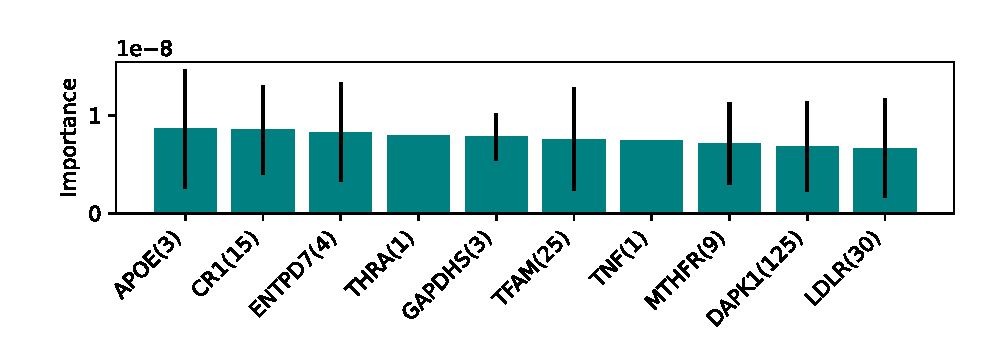
\includegraphics[width=0.85\textwidth]{images/biomarker-identification/alzgene-same-color.eps}
    \caption{Importance of each AlzGene group. The standard deviation and number of SNPs in each group is denoted by the line and the number next to the group name}\label{fig: AlzGene}
\end{figure}
% [Because of the dramatic increase in the prevalence of AD, the identification of effective biomarkers for the early diagnosis and treatment of AD in individuals at high risk to develop the disease is crucial.]
It is vital to identify AD relevant biomarkers for early detection and the treatment of people at high risk of developing AD. Despite the promising performance of deep neural networks, their predictions are notoriously difficult to interpret. To identify which biomarkers largely affect the predictions, we add the perturbation to the input data and observe the changes in prediction. The details of this identification method is described in supplementary. In Fig~\ref{fig: brain map} and Fig~\ref{fig: AlzGene}, we plot the importance distribution over the brain regions and AlzGene groups of SNPs. The AlzGene groups of SNPs have been constructed by the multiple genome-wide association studies listed on the website (\url{http://www.alzgene.org/}). From our model SAE, ventricular~\cite{carmichael2007ventricular}, hippocampus~\cite{mu2011adult}, and amygdala~\cite{poulin2011amygdala} are identified as important brain regions, and apolipoprotein E~\cite{kim2009role} and complement receptor 1~\cite{lambert2009genome} are identified as important AlzGene groups. The identified biomarkers have been shown in the literature to be related to AD, thus they provide substantial evidence that our approach can identify the biomarkers associated with AD.

% \begin{equation}\label{eq: SNPs identification}
% \begin{aligned}
%     &(\mathbf{x}_i^s)' = [x_{i, 1}^s, x_{i, 2}^s, \cdots, x_{i, m}^s + p_{i, m}, \cdots, x_{i, D_s}^s],\\
%     &\Delta\tilde{\mathbf{y}}_i = \| \psi_{pred}\bigl(\phi_{dynamic}(\mathbf{X}_i, \mathbf{M}_i, \mathbf{t}_i;\ \theta_{\phi}^d),\ \psi_{SNP}(\phi_{SNP}((\mathbf{x}_i^s)';\ \theta^s_{\phi});\ \theta^s_{\psi}),\ \mathbf{x}_i^b;\ \theta^p_{\psi}\bigr)\\
%     &- \psi_{pred}\bigl(\phi_{dynamic}(\mathbf{X}_i, \mathbf{M}_i, \mathbf{t}_i;\ \theta_{\phi}^d),\ \psi_{SNP}(\phi_{SNP}(\mathbf{x}_i^s;\ \theta^s_{\phi});\ \theta^s_{\psi}),\ \mathbf{x}_i^b;\ \theta^p_{\psi}\bigr)\|_1.
% \end{aligned}
% \end{equation}
% Finally, we plot top 15 most important features in Fig..
% \subsubsection{AD relevant imaging biomarkers}
% In Fig~\ref{fig: brain map}, we plot the importance distribution over the brain regions.
% % calculated by Eq.~\eqref{eq: neuroimaging identification}. 
% The identified regions have been shown in the literature to be related to AD. For example, the previous studies~\cite{carmichael2007ventricular} found that ventricular volume and its rate of change is related with vulnerability to cognitive decline and dementia. 
% % \cite{carmichael2007ventricular,jack2004comparison}
% They observe that the larger ventricles in healthy participants increase the probability to the progression of dementia-related disease in the future. The hippocampus is vulnerable to be damaged from AD~\cite{mu2011adult} and has been shown to affect long-term memory and spatial navigation in patients with AD. Finally, the amygdala region, also identified by our approach, is also severely affected by AD~\cite{poulin2011amygdala} and is associated with emotional response and decision-making.
% \subsubsection{AD relevant genetic biomarkers}
% We plot the importance distribution over the AlzGene groups of SNPs in Fig~\ref{fig: AlzGene}. The AlzGene groups of SNPs have been constructed by the multiple genome-wide association studies listed on the website (\url{http://www.alzgene.org/}). Apolipoprotein E (APOE) group is identified by our approach, and APOE genes involve in amyloid beta peptide (A$\beta$) aggregation and clearance~\cite{kim2009role}. The accumulation of A$\beta$ is commonly observed in the progress of AD~\cite{chen2017amyloid} and amyloid hypothesis suggests reasonable mechanism how the accumulation of A$\beta$ can result neuronal malfunction~\cite{hardy2002amyloid}. In addition, $\epsilon$4 allele of APOE gene increase risk factor for AD and decrease the age of AD onset~\cite{corder1993gene}. For complement receptor 1 (CR1) group, genome-wide analysis~\cite{lambert2009genome} reported CR1 association with late-onset AD. The subset of biomarkers identified in the FreeSurfer, VBM, and SNP modalities, provides substantial evidence that our approach can identify the biomarkers associated with AD.
% [Why multi-class classification? -> the different clinical actions are required for stage : AD, MCI, HC]
% even if very few samples are labeled.
\iffalse
An important characteristic of the present study was the use of a semi-supervised classification method for the AD conversion prediction in MCI subjects. The semi-supervised method (LDS) was shown to outperform its counterpart supervised method (SVM) in the design of MRI biomarker.
\fi
\section{Conclusion}
% In this work we aim to detect the Alzheimer's Disease (AD) progress in its early stage from the longitudinal multi-modal healthcare dataset, 
We present a semi-supervised enrichment learning method that integrates the longitudinal multi-modal dataset and is clinically applicable for use in real-time, automatic AD diagnosis. The novel LSTM autoencoder compresses longitudinal records with missing data into a fixed-length vectorial representation. Armed with this enriched representation, one can fully utilize the genotypic and phenotypic data. Our experiments show that our model outperforms competing predictive models. When combined with the perturbation based feature identification method, our model also discovers the neuroimaging and genetic biomarkers associated with AD, adding further value to our approach.
% Our model aims to detect the Alzheimer's Disease (AD) progress in its early stage from the longitudinal multi-modal healthcare dataset, which fits to the clinical applicability and can be used in a real-time automatic AD diagnosis.
% We have conducted extensive experiments on the Alzheimer's Disease Neuroimaging Initiative (ADNI) dataset~\cite{risacher2010longitudinal} and 
% achieved promising performance on multiclass AD progression prediction task with the various number of labeled samples. In our experiments with the proposed model, we identify the disease-relevant biomarkers through the perturbation based feature identification method.

{\small
\bibliographystyle{ieee_fullname}
\bibliography{bibliography}
}

\end{document}
